\begin{frame}{Theorie}
\textbf{Phänomen}: Ab einer Sprungtemperatur $T_{\mathup{C}}$ fällt elektrischer Widerstand auf $\SI{0}{\ohm}$ \\
\begin{itemize}
  \item
\end{itemize}


\textbf{Meißner-Ochsenfeld-Effekt}: Magnetfelder dringen nicht in den Supraleiter ein

\end{frame}



\begin{frame}{Meißner-Ochsenfeld-Effekt}
\begin{columns}
\begin{column}{0.49\textwidth}
  \begin{figure}
    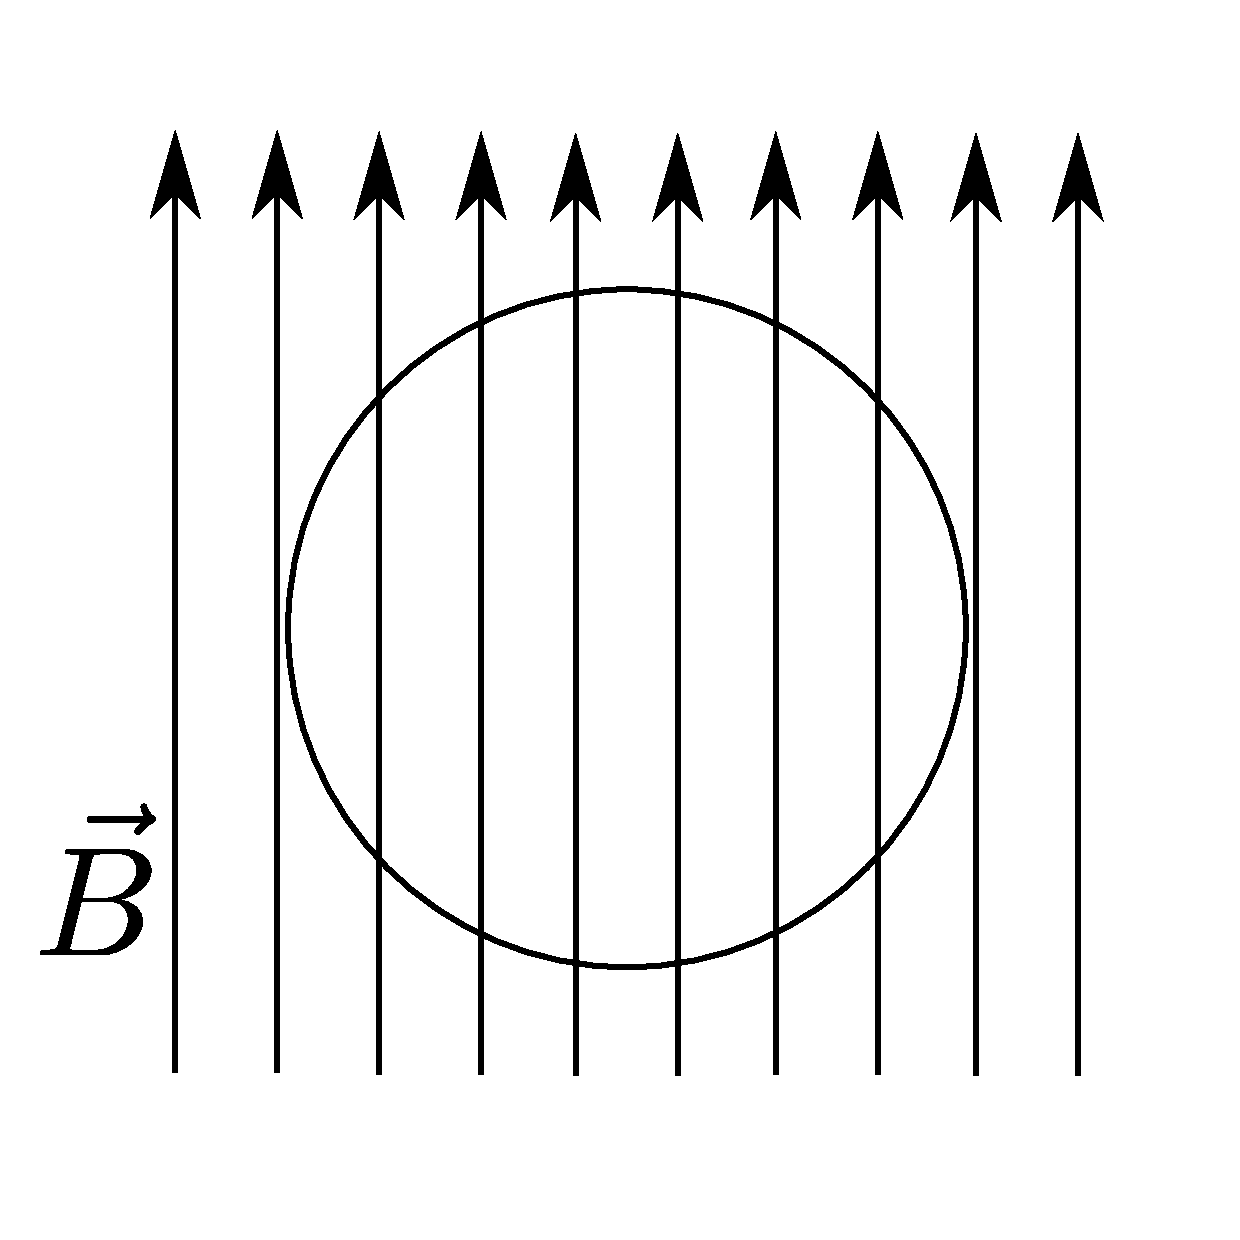
\includegraphics[width = \textwidth]{supra_1.pdf}
    \caption{Normale Leitung $T > T_{C}$}
    \label{}
  \end{figure}
\end{column}
\begin{column}{0.49\textwidth}
  \begin{figure}
    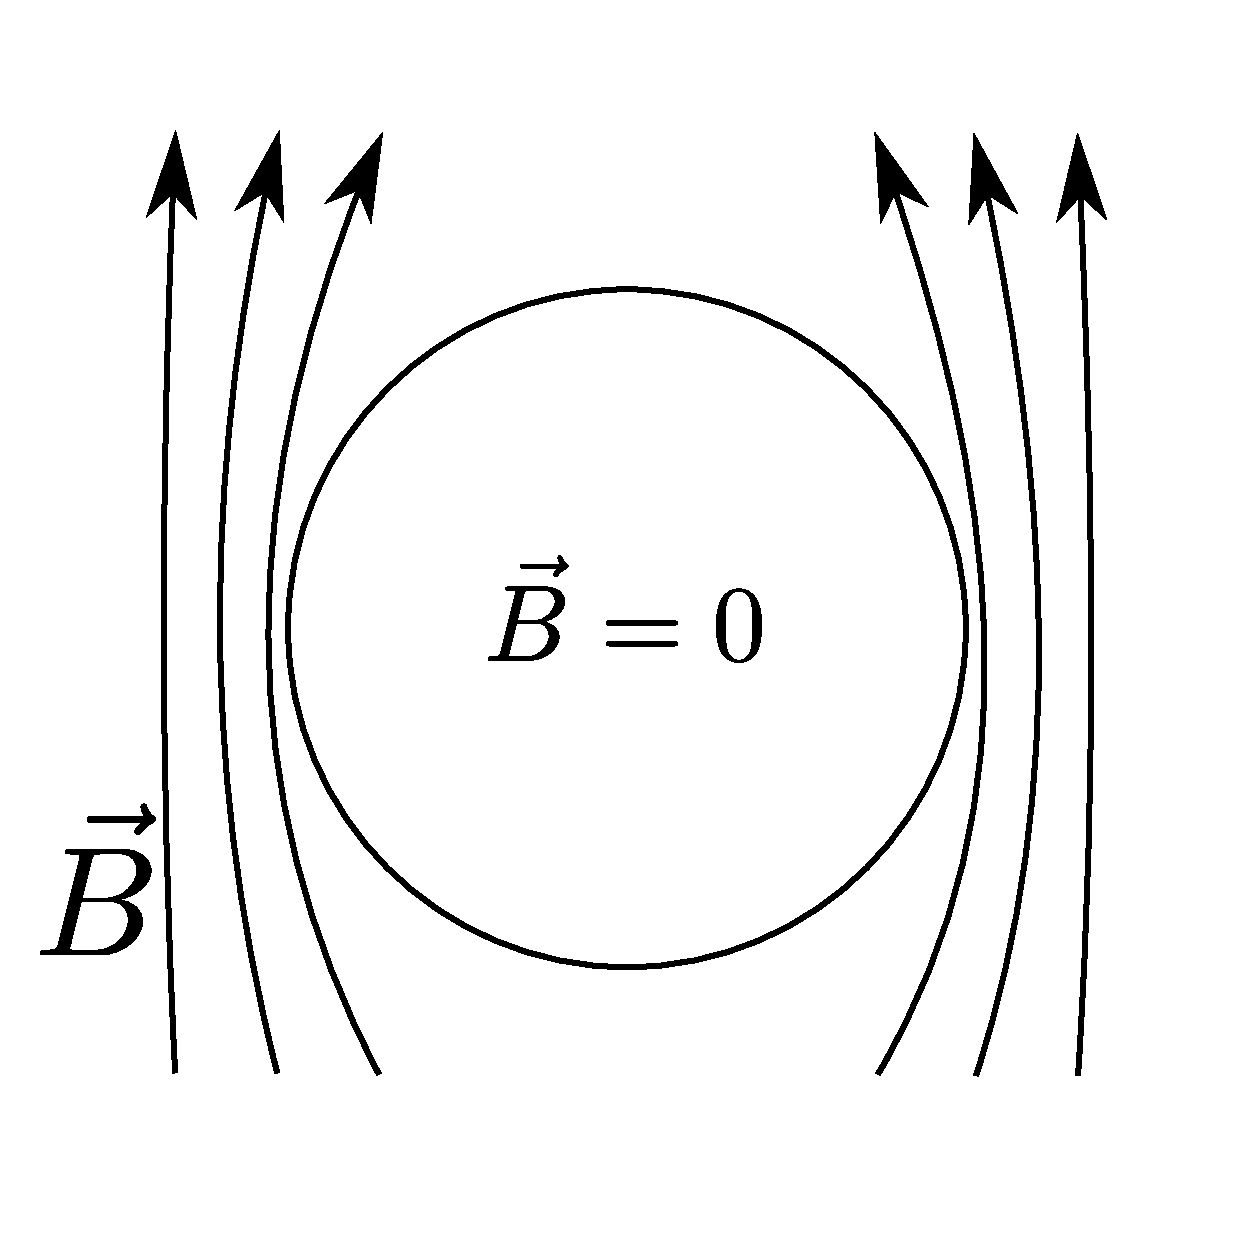
\includegraphics[width = \textwidth]{supra_2.pdf}
    \caption{Supraleitung $T < T_{C}$}
    \label{}
  \end{figure}
\end{column}
\end{columns}
\end{frame}
